% Options for packages loaded elsewhere
\PassOptionsToPackage{unicode}{hyperref}
\PassOptionsToPackage{hyphens}{url}
\PassOptionsToPackage{dvipsnames,svgnames,x11names}{xcolor}
%
\documentclass[
  letterpaper,
  DIV=11,
  numbers=noendperiod]{scrartcl}

\usepackage{amsmath,amssymb}
\usepackage{iftex}
\ifPDFTeX
  \usepackage[T1]{fontenc}
  \usepackage[utf8]{inputenc}
  \usepackage{textcomp} % provide euro and other symbols
\else % if luatex or xetex
  \usepackage{unicode-math}
  \defaultfontfeatures{Scale=MatchLowercase}
  \defaultfontfeatures[\rmfamily]{Ligatures=TeX,Scale=1}
\fi
\usepackage{lmodern}
\ifPDFTeX\else  
    % xetex/luatex font selection
\fi
% Use upquote if available, for straight quotes in verbatim environments
\IfFileExists{upquote.sty}{\usepackage{upquote}}{}
\IfFileExists{microtype.sty}{% use microtype if available
  \usepackage[]{microtype}
  \UseMicrotypeSet[protrusion]{basicmath} % disable protrusion for tt fonts
}{}
\makeatletter
\@ifundefined{KOMAClassName}{% if non-KOMA class
  \IfFileExists{parskip.sty}{%
    \usepackage{parskip}
  }{% else
    \setlength{\parindent}{0pt}
    \setlength{\parskip}{6pt plus 2pt minus 1pt}}
}{% if KOMA class
  \KOMAoptions{parskip=half}}
\makeatother
\usepackage{xcolor}
\setlength{\emergencystretch}{3em} % prevent overfull lines
\setcounter{secnumdepth}{-\maxdimen} % remove section numbering
% Make \paragraph and \subparagraph free-standing
\makeatletter
\ifx\paragraph\undefined\else
  \let\oldparagraph\paragraph
  \renewcommand{\paragraph}{
    \@ifstar
      \xxxParagraphStar
      \xxxParagraphNoStar
  }
  \newcommand{\xxxParagraphStar}[1]{\oldparagraph*{#1}\mbox{}}
  \newcommand{\xxxParagraphNoStar}[1]{\oldparagraph{#1}\mbox{}}
\fi
\ifx\subparagraph\undefined\else
  \let\oldsubparagraph\subparagraph
  \renewcommand{\subparagraph}{
    \@ifstar
      \xxxSubParagraphStar
      \xxxSubParagraphNoStar
  }
  \newcommand{\xxxSubParagraphStar}[1]{\oldsubparagraph*{#1}\mbox{}}
  \newcommand{\xxxSubParagraphNoStar}[1]{\oldsubparagraph{#1}\mbox{}}
\fi
\makeatother

\usepackage{color}
\usepackage{fancyvrb}
\newcommand{\VerbBar}{|}
\newcommand{\VERB}{\Verb[commandchars=\\\{\}]}
\DefineVerbatimEnvironment{Highlighting}{Verbatim}{commandchars=\\\{\}}
% Add ',fontsize=\small' for more characters per line
\usepackage{framed}
\definecolor{shadecolor}{RGB}{241,243,245}
\newenvironment{Shaded}{\begin{snugshade}}{\end{snugshade}}
\newcommand{\AlertTok}[1]{\textcolor[rgb]{0.68,0.00,0.00}{#1}}
\newcommand{\AnnotationTok}[1]{\textcolor[rgb]{0.37,0.37,0.37}{#1}}
\newcommand{\AttributeTok}[1]{\textcolor[rgb]{0.40,0.45,0.13}{#1}}
\newcommand{\BaseNTok}[1]{\textcolor[rgb]{0.68,0.00,0.00}{#1}}
\newcommand{\BuiltInTok}[1]{\textcolor[rgb]{0.00,0.23,0.31}{#1}}
\newcommand{\CharTok}[1]{\textcolor[rgb]{0.13,0.47,0.30}{#1}}
\newcommand{\CommentTok}[1]{\textcolor[rgb]{0.37,0.37,0.37}{#1}}
\newcommand{\CommentVarTok}[1]{\textcolor[rgb]{0.37,0.37,0.37}{\textit{#1}}}
\newcommand{\ConstantTok}[1]{\textcolor[rgb]{0.56,0.35,0.01}{#1}}
\newcommand{\ControlFlowTok}[1]{\textcolor[rgb]{0.00,0.23,0.31}{\textbf{#1}}}
\newcommand{\DataTypeTok}[1]{\textcolor[rgb]{0.68,0.00,0.00}{#1}}
\newcommand{\DecValTok}[1]{\textcolor[rgb]{0.68,0.00,0.00}{#1}}
\newcommand{\DocumentationTok}[1]{\textcolor[rgb]{0.37,0.37,0.37}{\textit{#1}}}
\newcommand{\ErrorTok}[1]{\textcolor[rgb]{0.68,0.00,0.00}{#1}}
\newcommand{\ExtensionTok}[1]{\textcolor[rgb]{0.00,0.23,0.31}{#1}}
\newcommand{\FloatTok}[1]{\textcolor[rgb]{0.68,0.00,0.00}{#1}}
\newcommand{\FunctionTok}[1]{\textcolor[rgb]{0.28,0.35,0.67}{#1}}
\newcommand{\ImportTok}[1]{\textcolor[rgb]{0.00,0.46,0.62}{#1}}
\newcommand{\InformationTok}[1]{\textcolor[rgb]{0.37,0.37,0.37}{#1}}
\newcommand{\KeywordTok}[1]{\textcolor[rgb]{0.00,0.23,0.31}{\textbf{#1}}}
\newcommand{\NormalTok}[1]{\textcolor[rgb]{0.00,0.23,0.31}{#1}}
\newcommand{\OperatorTok}[1]{\textcolor[rgb]{0.37,0.37,0.37}{#1}}
\newcommand{\OtherTok}[1]{\textcolor[rgb]{0.00,0.23,0.31}{#1}}
\newcommand{\PreprocessorTok}[1]{\textcolor[rgb]{0.68,0.00,0.00}{#1}}
\newcommand{\RegionMarkerTok}[1]{\textcolor[rgb]{0.00,0.23,0.31}{#1}}
\newcommand{\SpecialCharTok}[1]{\textcolor[rgb]{0.37,0.37,0.37}{#1}}
\newcommand{\SpecialStringTok}[1]{\textcolor[rgb]{0.13,0.47,0.30}{#1}}
\newcommand{\StringTok}[1]{\textcolor[rgb]{0.13,0.47,0.30}{#1}}
\newcommand{\VariableTok}[1]{\textcolor[rgb]{0.07,0.07,0.07}{#1}}
\newcommand{\VerbatimStringTok}[1]{\textcolor[rgb]{0.13,0.47,0.30}{#1}}
\newcommand{\WarningTok}[1]{\textcolor[rgb]{0.37,0.37,0.37}{\textit{#1}}}

\providecommand{\tightlist}{%
  \setlength{\itemsep}{0pt}\setlength{\parskip}{0pt}}\usepackage{longtable,booktabs,array}
\usepackage{calc} % for calculating minipage widths
% Correct order of tables after \paragraph or \subparagraph
\usepackage{etoolbox}
\makeatletter
\patchcmd\longtable{\par}{\if@noskipsec\mbox{}\fi\par}{}{}
\makeatother
% Allow footnotes in longtable head/foot
\IfFileExists{footnotehyper.sty}{\usepackage{footnotehyper}}{\usepackage{footnote}}
\makesavenoteenv{longtable}
\usepackage{graphicx}
\makeatletter
\newsavebox\pandoc@box
\newcommand*\pandocbounded[1]{% scales image to fit in text height/width
  \sbox\pandoc@box{#1}%
  \Gscale@div\@tempa{\textheight}{\dimexpr\ht\pandoc@box+\dp\pandoc@box\relax}%
  \Gscale@div\@tempb{\linewidth}{\wd\pandoc@box}%
  \ifdim\@tempb\p@<\@tempa\p@\let\@tempa\@tempb\fi% select the smaller of both
  \ifdim\@tempa\p@<\p@\scalebox{\@tempa}{\usebox\pandoc@box}%
  \else\usebox{\pandoc@box}%
  \fi%
}
% Set default figure placement to htbp
\def\fps@figure{htbp}
\makeatother
% definitions for citeproc citations
\NewDocumentCommand\citeproctext{}{}
\NewDocumentCommand\citeproc{mm}{%
  \begingroup\def\citeproctext{#2}\cite{#1}\endgroup}
\makeatletter
 % allow citations to break across lines
 \let\@cite@ofmt\@firstofone
 % avoid brackets around text for \cite:
 \def\@biblabel#1{}
 \def\@cite#1#2{{#1\if@tempswa , #2\fi}}
\makeatother
\newlength{\cslhangindent}
\setlength{\cslhangindent}{1.5em}
\newlength{\csllabelwidth}
\setlength{\csllabelwidth}{3em}
\newenvironment{CSLReferences}[2] % #1 hanging-indent, #2 entry-spacing
 {\begin{list}{}{%
  \setlength{\itemindent}{0pt}
  \setlength{\leftmargin}{0pt}
  \setlength{\parsep}{0pt}
  % turn on hanging indent if param 1 is 1
  \ifodd #1
   \setlength{\leftmargin}{\cslhangindent}
   \setlength{\itemindent}{-1\cslhangindent}
  \fi
  % set entry spacing
  \setlength{\itemsep}{#2\baselineskip}}}
 {\end{list}}
\usepackage{calc}
\newcommand{\CSLBlock}[1]{\hfill\break\parbox[t]{\linewidth}{\strut\ignorespaces#1\strut}}
\newcommand{\CSLLeftMargin}[1]{\parbox[t]{\csllabelwidth}{\strut#1\strut}}
\newcommand{\CSLRightInline}[1]{\parbox[t]{\linewidth - \csllabelwidth}{\strut#1\strut}}
\newcommand{\CSLIndent}[1]{\hspace{\cslhangindent}#1}

\KOMAoption{captions}{tableheading}
\makeatletter
\@ifpackageloaded{tcolorbox}{}{\usepackage[skins,breakable]{tcolorbox}}
\@ifpackageloaded{fontawesome5}{}{\usepackage{fontawesome5}}
\definecolor{quarto-callout-color}{HTML}{909090}
\definecolor{quarto-callout-note-color}{HTML}{0758E5}
\definecolor{quarto-callout-important-color}{HTML}{CC1914}
\definecolor{quarto-callout-warning-color}{HTML}{EB9113}
\definecolor{quarto-callout-tip-color}{HTML}{00A047}
\definecolor{quarto-callout-caution-color}{HTML}{FC5300}
\definecolor{quarto-callout-color-frame}{HTML}{acacac}
\definecolor{quarto-callout-note-color-frame}{HTML}{4582ec}
\definecolor{quarto-callout-important-color-frame}{HTML}{d9534f}
\definecolor{quarto-callout-warning-color-frame}{HTML}{f0ad4e}
\definecolor{quarto-callout-tip-color-frame}{HTML}{02b875}
\definecolor{quarto-callout-caution-color-frame}{HTML}{fd7e14}
\makeatother
\makeatletter
\@ifpackageloaded{caption}{}{\usepackage{caption}}
\AtBeginDocument{%
\ifdefined\contentsname
  \renewcommand*\contentsname{Table of contents}
\else
  \newcommand\contentsname{Table of contents}
\fi
\ifdefined\listfigurename
  \renewcommand*\listfigurename{List of Figures}
\else
  \newcommand\listfigurename{List of Figures}
\fi
\ifdefined\listtablename
  \renewcommand*\listtablename{List of Tables}
\else
  \newcommand\listtablename{List of Tables}
\fi
\ifdefined\figurename
  \renewcommand*\figurename{Figure}
\else
  \newcommand\figurename{Figure}
\fi
\ifdefined\tablename
  \renewcommand*\tablename{Table}
\else
  \newcommand\tablename{Table}
\fi
}
\@ifpackageloaded{float}{}{\usepackage{float}}
\floatstyle{ruled}
\@ifundefined{c@chapter}{\newfloat{codelisting}{h}{lop}}{\newfloat{codelisting}{h}{lop}[chapter]}
\floatname{codelisting}{Listing}
\newcommand*\listoflistings{\listof{codelisting}{List of Listings}}
\makeatother
\makeatletter
\makeatother
\makeatletter
\@ifpackageloaded{caption}{}{\usepackage{caption}}
\@ifpackageloaded{subcaption}{}{\usepackage{subcaption}}
\makeatother

\usepackage{bookmark}

\IfFileExists{xurl.sty}{\usepackage{xurl}}{} % add URL line breaks if available
\urlstyle{same} % disable monospaced font for URLs
\hypersetup{
  pdftitle={Manchu Learning: A Manchu-English Machine Translation Project},
  colorlinks=true,
  linkcolor={blue},
  filecolor={Maroon},
  citecolor={Blue},
  urlcolor={Blue},
  pdfcreator={LaTeX via pandoc}}


\title{Manchu Learning: A Manchu-English Machine Translation Project}
\usepackage{etoolbox}
\makeatletter
\providecommand{\subtitle}[1]{% add subtitle to \maketitle
  \apptocmd{\@title}{\par {\large #1 \par}}{}{}
}
\makeatother
\subtitle{DSAN6600 Neural Networks and Deep Learning}
\author{Christy Hsu}
\date{}

\begin{document}
\maketitle


\subsection{Introduction}\label{introduction}

This project is an attempt to try out a Neural Machine Translation
approach for the challenging task of Manchu-English translation.

\begin{itemize}
\tightlist
\item
  Keywords: Neural Machine Translation, Data Curation, In-Context
  Machine Translation, Endangered Language
\end{itemize}

\begin{tcolorbox}[enhanced jigsaw, opacitybacktitle=0.6, arc=.35mm, titlerule=0mm, colframe=quarto-callout-note-color-frame, title=\textcolor{quarto-callout-note-color}{\faInfo}\hspace{0.5em}{The Language Manchu}, colbacktitle=quarto-callout-note-color!10!white, coltitle=black, rightrule=.15mm, toprule=.15mm, leftrule=.75mm, bottomtitle=1mm, breakable, toptitle=1mm, left=2mm, opacityback=0, bottomrule=.15mm, colback=white]

\paragraph{Our Goal and the challenges along the
way}\label{our-goal-and-the-challenges-along-the-way}

\pandocbounded{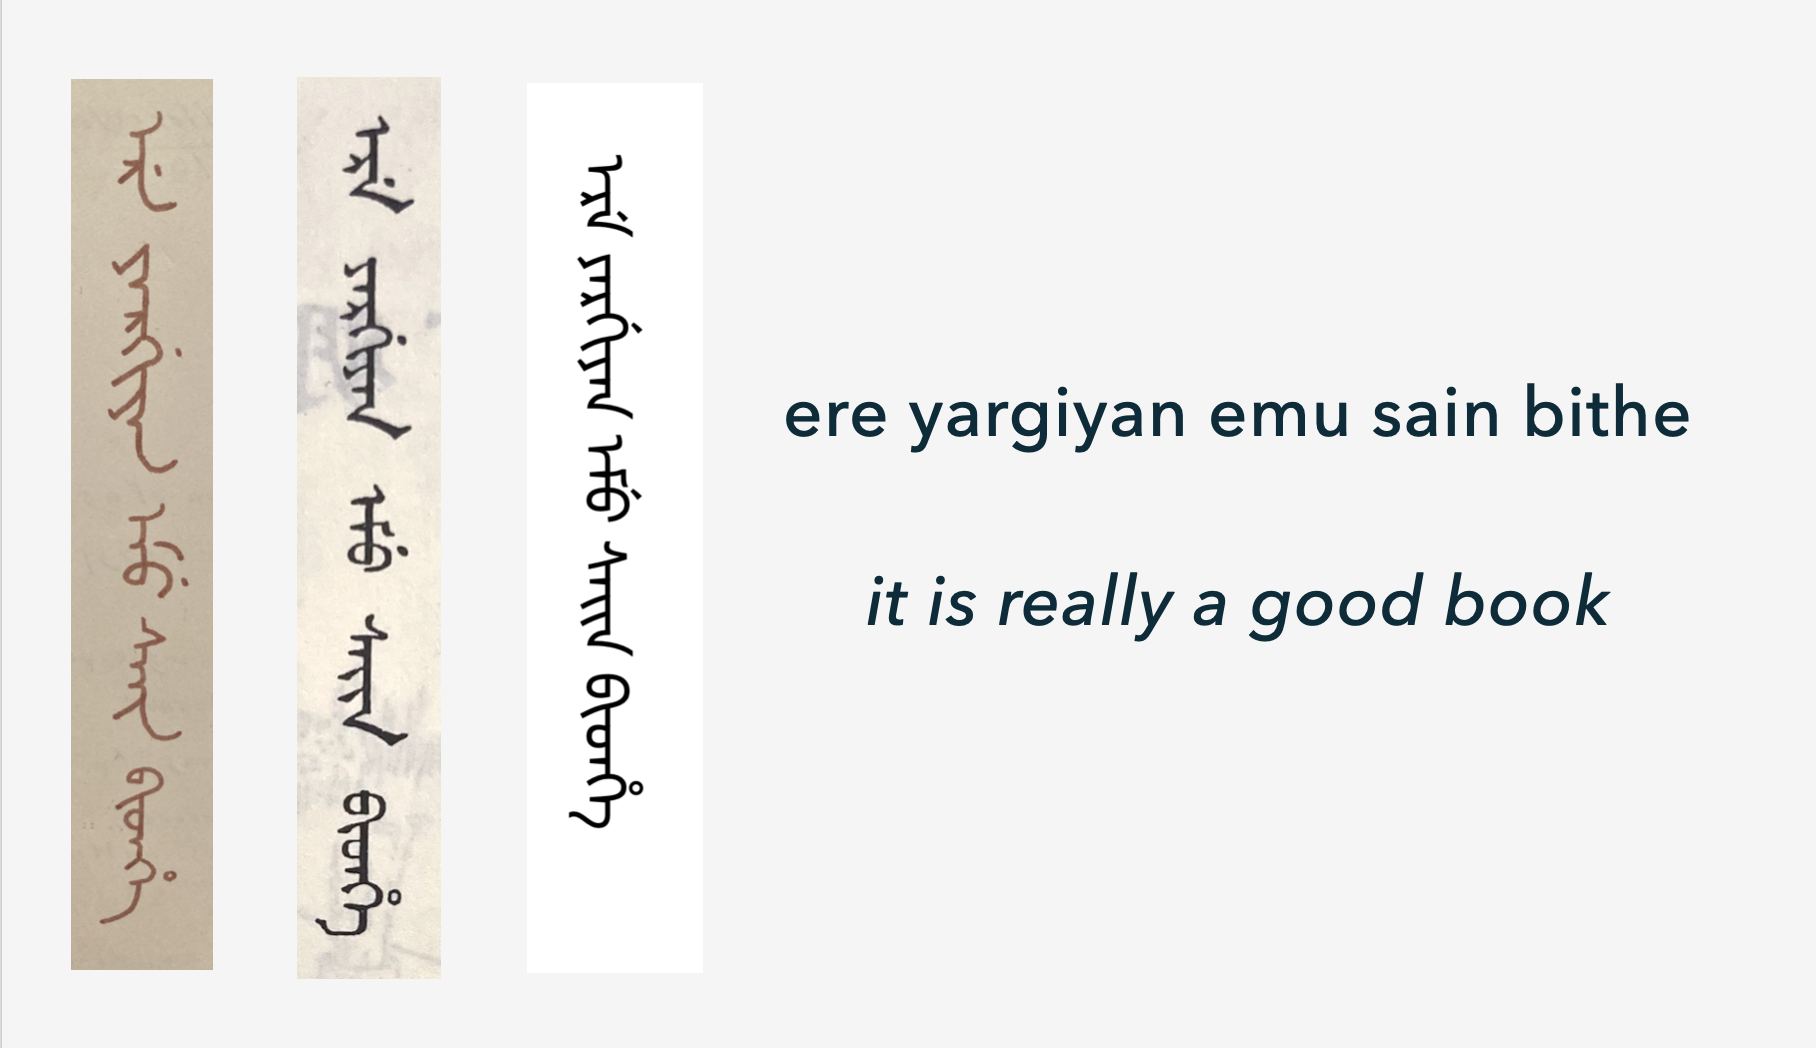
\includegraphics[keepaspectratio]{images/manchu-steps.png}}

\begin{enumerate}
\def\labelenumi{\arabic{enumi}.}
\tightlist
\item
  Language in danger: Manchu is often treated as Latin, mainly learned
  to read historical documents, but unlike Latin, it still has a spoken
  tradition today. In the \textbf{Qapqal Xibe Autonomous County} in
  Xinjiang, where its use is part of deliberate preservation efforts,
  taken by the Xibe people in the name of Xibe (Sibe) language
\item
  Digitization challenges: As some might have observed that the Manchu
  writing system is very far from that of English or the most common
  writing system in the world. First, the direction, in \textbf{columns}
  and from left to right, similar to Arabic rotated 90 degrees
  counter-clockwise. Second, Manchu script (alphabets) can be described
  as \textbf{IMFI} script whih letters can take on more than four
  different shapes depending on where they appear in the word or in
  isolation. This complicated the picture for OCR, due to the extra work
  on letter segmentation.
\item
  Transliteration
\item
  Traslation
\end{enumerate}

\end{tcolorbox}

\subsection{Literature Review}\label{literature-review}

In this section, I want to briefly talk about the three papers that
introduced me to the task of Manchu Machine Translation and I helped
shape my methods and approaches in this project. These studies, in their
distinctive ways engaged the Manchu Language revitalization effort in
the broader dialogue of Neural Machine Translation in low-resource
settings.

\subparagraph[Seo et al., \emph{``Mergen: The First Manchu-Korean
Machine Translation Model Trained on Augmented
Data.''}]{\texorpdfstring{Seo et al., \emph{``Mergen: The First
Manchu-Korean Machine Translation Model Trained on Augmented
Data.''}\footnote{Seo et al.
  (\citeproc{ref-seoMergenFirstManchuKorean2024}{2024})}}{Seo et al., ``Mergen: The First Manchu-Korean Machine Translation Model Trained on Augmented Data.''}}\label{seo-et-al.-mergen-the-first-manchu-korean-machine-translation-model-trained-on-augmented-data.}

This paper introduces us the challenges of developing the typically
data-driven Nueral Machine Translation models for Manchu, which suffers
from scarcity (an extreme one) of parallel data --not only just in their
case of Manchu-Korean translation, but generally. They thus come up with
an innovative data augmentation strategy based on \textbf{word
replacement}, where lexical similarity is determined using GloVe
embeddings of dictionary items. By augmenting the parallel corpus in
this way, they witness a significant improvement of the BLEU score of
their seq2seq model, from 0 to 38 as number of sentence pairs grows from
20K to 179K.

\subparagraph[Lee et al., \emph{``ManNER \& ManPOS: Pioneering NLP for
Endangered Manchu Language.''}]{\texorpdfstring{Lee et al.,
\emph{``ManNER \& ManPOS: Pioneering NLP for Endangered Manchu
Language.''}\footnote{Lee et al.
  (\citeproc{ref-leeManNERManPOSPioneering2024}{2024})}}{Lee et al., ``ManNER \& ManPOS: Pioneering NLP for Endangered Manchu Language.''}}\label{lee-et-al.-manner-manpos-pioneering-nlp-for-endangered-manchu-language.}

This study, continuing their line of work, this team of researcher with
their data augmentation technique further contributed by training from
scratch the Manchu Langauge Model \textbf{manchuBERT} and releasing the
model on Hugging Face. They then use the manchuBERT as the starting
point for developing NER and POS tagging for Manchu, the strong
performance of these downstream NLP modeling in turn provides evidence
that manchuBERT langauge model indeed learned to be a robust encoder for
Manchu.

\paragraph[Pei et al., \emph{Understanding In-Context Machine
Translation for Low-Resource Languages: A Case Study on
Manchu}]{\texorpdfstring{Pei et al., \emph{Understanding In-Context
Machine Translation for Low-Resource Languages: A Case Study on
Manchu}\footnote{Pei, Liu, Lin, Yvon, and Schuetze
  (\citeproc{ref-pei-etal-2025-understanding}{2025})}}{Pei et al., Understanding In-Context Machine Translation for Low-Resource Languages: A Case Study on Manchu}}\label{pei-et-al.-understanding-in-context-machine-translation-for-low-resource-languages-a-case-study-on-manchu}

The third paper also devotes to the discussion of the prospect of
low-resource machine translation, but approach the problem from a
different angle. Rather than focusing on model architectural
modifications or data augmentation, they get themselves around to think
about how \textbf{human-curated linguistic knowledge}, such as
dictionaries and grammar books can help in this picture. Specifically,
how these linguistic resources can be instilled to pre-trained LLM and
leverage their in-context learning (\textbf{ICL}) capability to machine
translation of languages they are not trained on. Through experiment
designs they systematically examine the effect of different linguistic
information, and arrive at the conclusion that, dictionaries that
comprehensively covers lexical meanings, suffix explanations, and
morpheme collocation info can effectively improve translation quality,
the same can parallel examples.

\subsection{Data}\label{data}

\subsubsection{Data Collection}\label{data-collection}

The data used in this project is one small but carefully examined
Manchu-English parallel dataset. I chose the renowned novel
\textbf{\emph{The Dream of the Red Chamber}} written in classical
Chinese by Cao Xueqin (published in the 1790s Qing China)\footnote{the
  novel was written in ``Written Vernacular Chinese'', but still not
  that as explicit as modern Chinese}, in specific, the novel's Manchu
translation(曹雪芹
(\citeproc{ref-CaoXueQinHongLouMengXiBoWen1993}{1993})) and English
translation (Cao (\citeproc{ref-caoHungLouMeng2006}{2006})) With the
hope that translators of this canonical literature had stronger emphasis
on fidelity to the original text thus expecting it to be relatively
easier for me to find sentence-level alignment that would help me a lot
in building my language pairs

Here, I present some key distributions of my dataset:

Sentence Length:

\begin{itemize}
\tightlist
\item
  Manchu: 5.38 words per sentence in average
\item
  English: 7,73 words per sentence in average
\end{itemize}

\pandocbounded{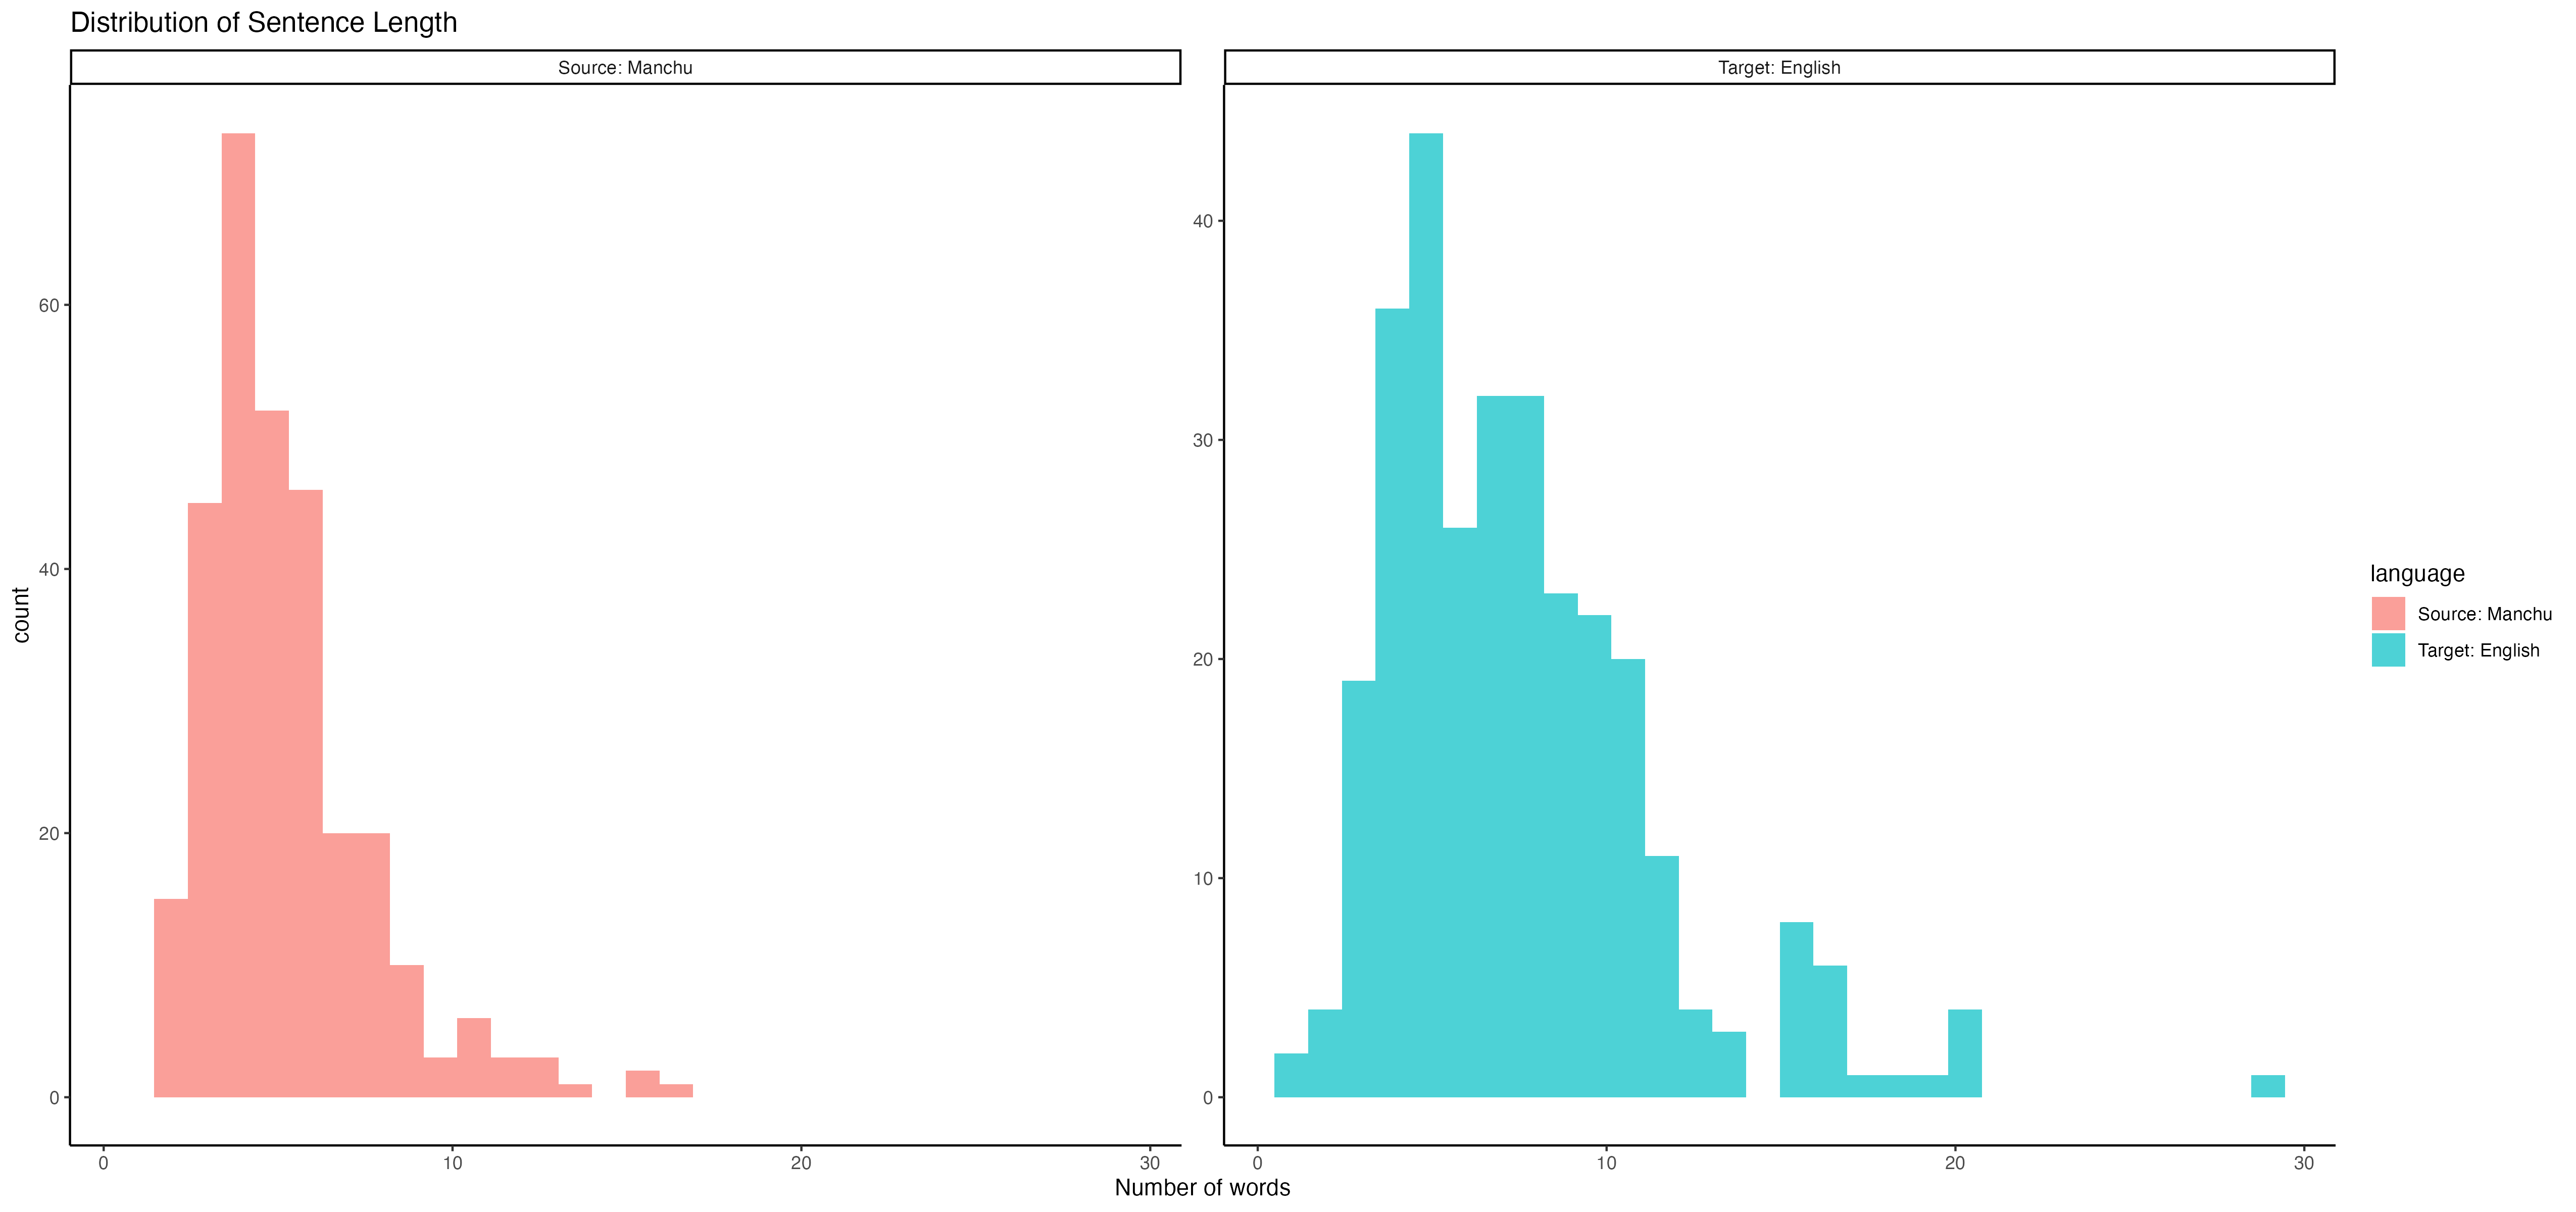
\includegraphics[keepaspectratio]{images/sent-plot.png}}

Vocabulary Size:

\begin{itemize}
\tightlist
\item
  Manchu: 700 distinct words
\item
  English: 669 distinct words
\end{itemize}

\pandocbounded{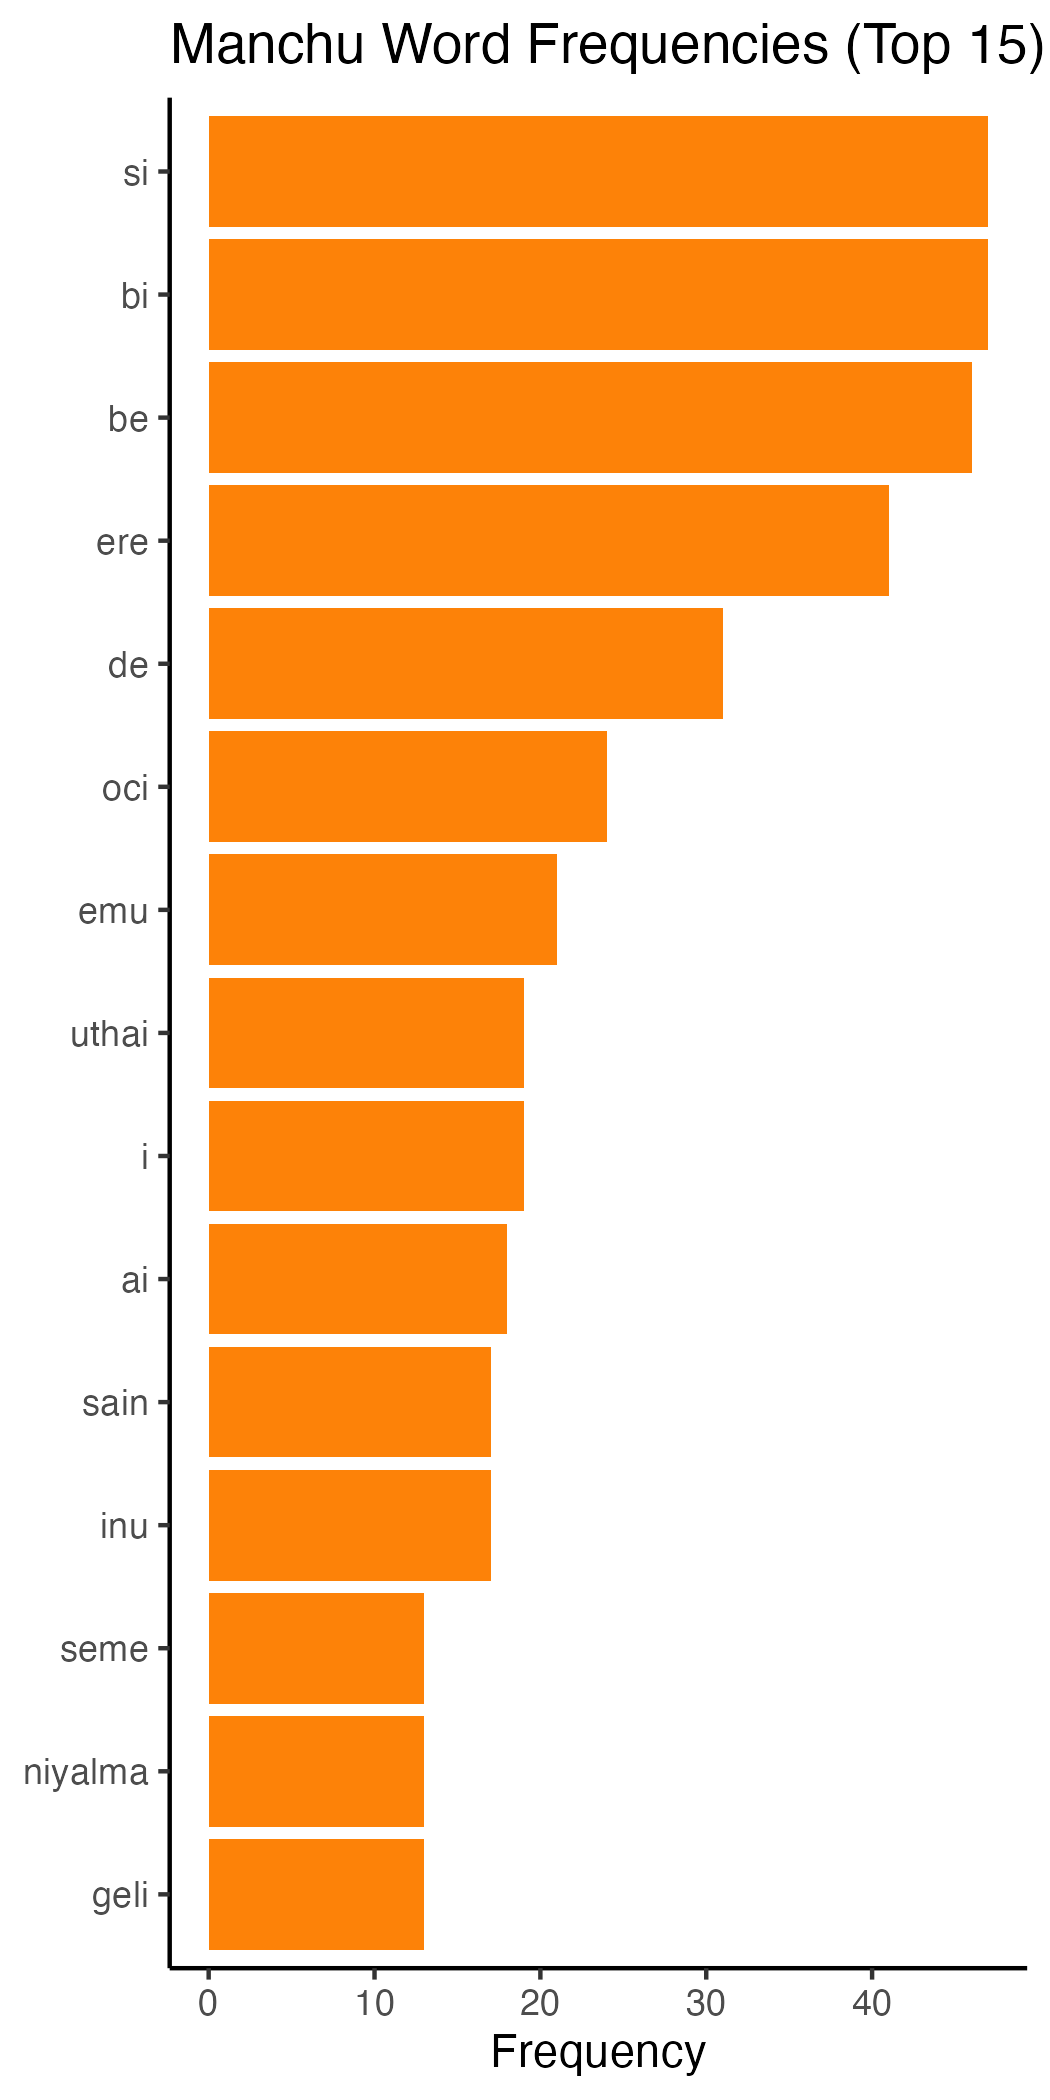
\includegraphics[keepaspectratio]{images/mnc-word-freq-plot.png}}

\pandocbounded{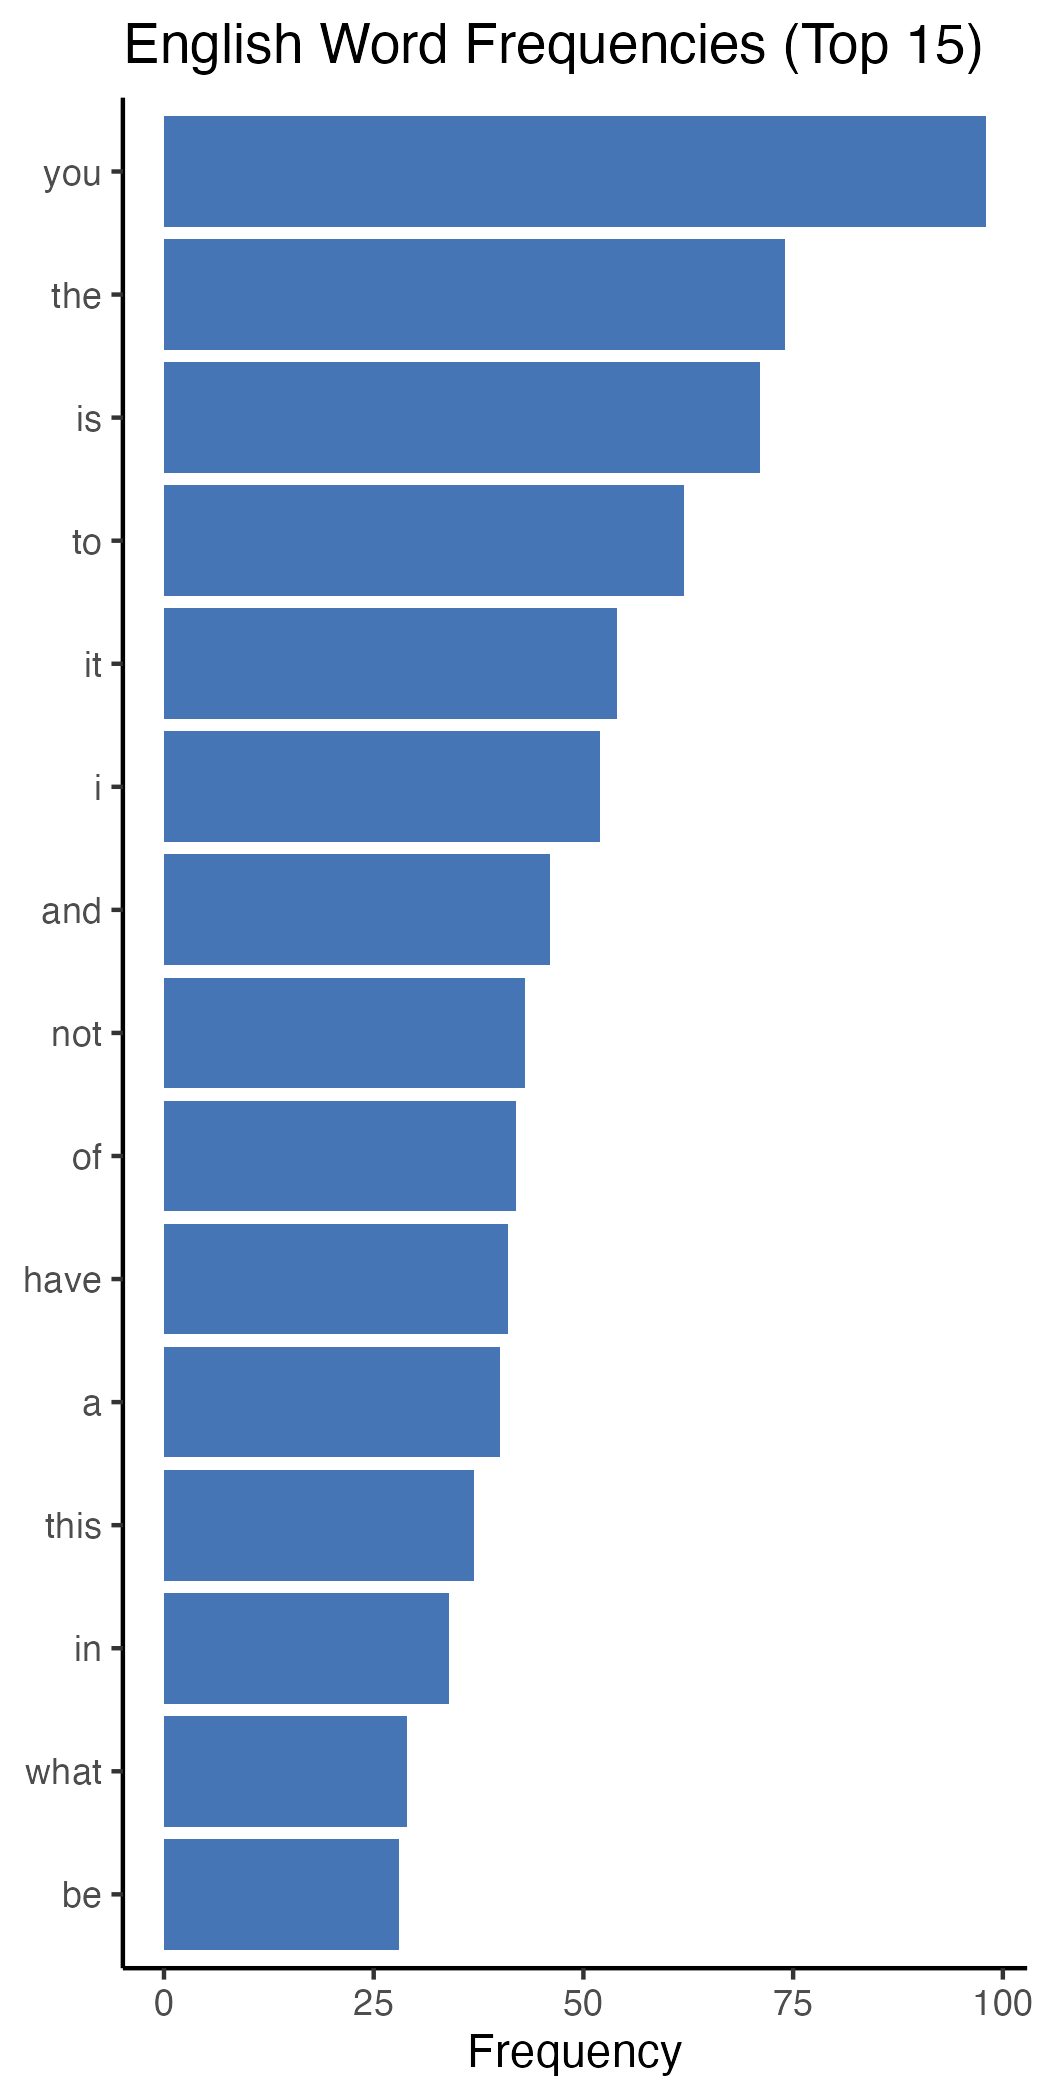
\includegraphics[keepaspectratio]{images/en-word-freq-plot.png}}

\paragraph{Data Split}\label{data-split}

I reserved 12.5\% for validation (37 rows), as for the other 38 rows for
testing, which remains 225 rows for training. Given the very limited
size of our data, and the often large size of training parameters in our
neural models, regularization and monitoring validation loss are both
very crucial concerns in the training process.\footnote{a better and
  definitely doable robustness test is to implement k-fold cross
  validation so as to eliminate the effect of data splitting for small
  sample}

\subsubsection{Data Preprocessing}\label{data-preprocessing}

\paragraph{Text cleaning and
normalization}\label{text-cleaning-and-normalization}

For simplicity, I removed all the punctuations, and all sentences are
converted to lowercase.

\begin{tcolorbox}[enhanced jigsaw, opacitybacktitle=0.6, arc=.35mm, titlerule=0mm, colframe=quarto-callout-note-color-frame, title=\textcolor{quarto-callout-note-color}{\faInfo}\hspace{0.5em}{The issue of Transliteration Alignment}, colbacktitle=quarto-callout-note-color!10!white, coltitle=black, rightrule=.15mm, toprule=.15mm, leftrule=.75mm, bottomtitle=1mm, breakable, toptitle=1mm, left=2mm, opacityback=0, bottomrule=.15mm, colback=white]

One challenge I encountered in the data preparation phase is around the
issue of transliteration, and I found it worth recording, so I would
like to share it here. The transliteration system that I was using
initially for my self-curated dataset is the \textbf{Möllendorff-Norman}
system, because this is the one our Manchu professor taught, and also
one of the most used system.

Later in an attempt of harvesting from the pre-trained manchuBERT, I
found in the \emph{Mergen (2024)} paper statements that they use
\textbf{Abkai transliteration}, so I converted my dataset into Abkai
only to find out that they not quite entirely adopt this system. To
clarify this, and because the datasets they disclosed in the github
repository are the test ones, thus I did a small experiment with the
manchuBERT as masked language model. After inputting some sentences with
mask tokens, the outputs of manchuBERT revealed that they actually use a
hybrid system for transliteration, for example, the model represents the
sixth Manchu vowel using \texttt{v} rather than the Norman \texttt{ū};
uses \texttt{x} instead of the Norman \texttt{š}, which seems to be
aligning to the Abkai system. At the same time, it employs Norman
\texttt{c} rather than the Abkai-preferred \texttt{q}.

Regarding to these observations, I re-romanized the Manchu side of my
data to ensure the alignment of the one manchuBERT learnt. I think this
transliteration alignment process that I underwent actually highlights a
non-trivial challenge in obtaining and integrating online Manchu
resources, when without a standardized transliteration system, languages
that use non-Latin scripts are going to suffer, or will require
additional attention in the data preprocessing stage.

\end{tcolorbox}

\paragraph{Tokenization}\label{tokenization}

Different ways for tokenizations are implemented for my four MT
attempts. I would like to provide a brief illustration in this section
before we go into the models.

In \emph{Attempt 1}, tokenization was done by splitting our sentences by
white spaces, thus, a word-level tokenization.\footnote{with four
  additional tokens, , , ,} As for \emph{Attempt 2}, to correctly map to
manchuBERT, I use the AutoTokenizer from Hugging Face transformer
library to retrieve the tokenizer of our pre-trained model. And as
stated in the paper, the tokenization they applied is
\textbf{WordPiece}; in the English output part the bert-base-ubcased
tokenizer was applied.\footnote{with manually handling and}In
\emph{Attempt 3}, I continue to use the manchuBERT tokenizer for Manchu
source sentences; the English counterpart uses the SentencePiece
tokenization, which does the \textbf{subword} segmentation, and I have
to additionally specify the tokenizer to translate into English.
Finally, \emph{Attempt 4}, the sentence was feed to google colab AI
directly.

\subsection{Approaches}\label{approaches}

\subsubsection{\texorpdfstring{\emph{Attempt 1: 2 GRUs} -- Seq2seq
Network with
Attention}{Attempt 1: 2 GRUs -- Seq2seq Network with Attention}}\label{attempt-1-2-grus-seq2seq-network-with-attention}

This is the baseline model I go for, and I reference directly to the
Pytorch tutorial for the implementation from scratch({``{NLP From
Scratch}: {Translation} with a {Sequence} to {Sequence Network} and
{Attention} --- {PyTorch Tutorials} 2.9.0+cu128 Documentation''}
(\citeproc{ref-NLPScratchTranslation}{n.d.})), and also because it has a
similar structure to the descriptions in the Mergen paper(Seo et al.
(\citeproc{ref-seoMergenFirstManchuKorean2024}{2024}))

Model Architecture:

\begin{itemize}
\tightlist
\item
  The sequence-to-sequence model involves two RNNs, carried out as
  \textbf{Gated Recurrent Units}. Our first GRU did the encoder job, and
  the second GRU has a twist of the attention weights calculation in the
  decoding.\footnote{the attention mechanism is the \textbf{additive
    Bahdanau attention}, one way of looking at this mechanism, in the
    context of neural machine translation, is that it helps in many ways
    to the ability to deal with word ordering of our languages, and
    order the varying lengths of the sentences.}
\end{itemize}

Hyperparameters:

\begin{itemize}
\tightlist
\item
  Learning Rate = 0.001
\item
  Embedding size = 256
\item
  Hidden Size = 512
\item
  Dropout Rate = 0.2
\item
  Epochs = 20
\end{itemize}

\subsubsection{\texorpdfstring{\emph{Attempt 2: Frozen ManchuBERT + LSTM
Decoder}}{Attempt 2: Frozen ManchuBERT + LSTM Decoder}}\label{attempt-2-frozen-manchubert-lstm-decoder}

Model Designs:

\begin{itemize}
\tightlist
\item
  My second attempt reflects the representation-level transfer learning,
  which I use the \texttt{Automodel} class from transformers library to
  load the \textbf{manchuBERT} model configuration from Hugging Face,
  and then I use the method \texttt{from\_pretrained()} to acquire the
  model parameters. As provided in the documentation (Seo et al.
  (\citeproc{ref-seoMergenFirstManchuKorean2024}{2024})), manchuBERT is
  a language model trained on more than 5.2 M monolingual Manchu
  sentences\footnote{195,611 monolingual Manchu sentences before data
    augmentation} And the embedding vector is of 768 length. With the
  help of manchuBERT our raw Manchu input can be transformed into rich
  and context-aware representation space, as an encoder I pair it with
  an LSTM decoder for our downstream translation task.
\end{itemize}

Hyperparameters:

\begin{itemize}
\tightlist
\item
  Learning Rate = 2e-4
\item
  Embedding size = 256
\item
  Hidden Size = 512
\item
  Number of Layers = 2
\item
  Dropout Rate = 0.2
\item
  Epochs = 50
\end{itemize}

\subsubsection{\texorpdfstring{\emph{Attempt 3: manchuBERT \&
mBART}}{Attempt 3: manchuBERT \& mBART}}\label{attempt-3-manchubert-mbart}

Model Designs:

\begin{itemize}
\tightlist
\item
  The new things introduce in our Attempt 3 is that we now pass our
  encodings to the \textbf{mBART},\footnote{One of the key contributions
    of the mBART model is that it is proven to be conducive to
    translation of even the languages unseen by the model to fluent
    English sentences} the pre-trained, \textbf{end-to-end} multilingual
  to English model there to help us getting from encoded Manchu to
  sensical English sentences.(Liu et al.
  (\citeproc{ref-liuMultilingualDenoisingPretraining2020}{2020}))
\end{itemize}

Hyperparameters:

\begin{itemize}
\tightlist
\item
  Learning Rate = 3e-5
\item
  Epochs = 30
\end{itemize}

\subsubsection{\texorpdfstring{\emph{Attempt 4: Norman Dictionary +
Google Colab AI} -- In-Context Machine
Translation}{Attempt 4: Norman Dictionary + Google Colab AI -- In-Context Machine Translation}}\label{attempt-4-norman-dictionary-google-colab-ai-in-context-machine-translation}

Experiment Designs

\begin{itemize}
\tightlist
\item
  Our last attempt was primarily inspired by the ICL Machine Translation
  paper\footnote{Pei, Liu, Lin, Yvon, and Schütze
    (\citeproc{ref-pei2025understandingincontextmachinetranslation}{2025})}
  The linguistic resource explored is \emph{The Comprehensive
  Manchu-English Dictionary} from Jerry Norman(Norman
  (\citeproc{ref-normanComprehensiveManchuEnglishDictionary2013}{2013}))
  Step by step, I first parse the dictioanry into
  \texttt{item}-\texttt{meaning} pairs of 21K, and I retrieve the
  vocabularies from our source Manchu sentence and incorporate the
  dictionary info as part of the translation prompt
\item
  One more special account for Attempt 4 is that rather than directly
  encipher our source to eliminate the prior knowledge of our LLM, I
  introduce some controls to the experiment by speicify that the task is
  Manchu-to-English or not specifying the target language, or create a
  substitute such as ``Anchum'' language in the prompt.
\end{itemize}

Prompt example:

\begin{Shaded}
\begin{Highlighting}[]

\NormalTok{Please help me translate the following input sentence into English}
\NormalTok{For the translation task, you are given the word by word mapping}
\NormalTok{from the \{source language\} words to the \{target language\} words}

\NormalTok{        Please try your best to translate, it’s okay }\ControlFlowTok{if}
\NormalTok{        your translation is bad. Do not refuse to try it.}
\NormalTok{        I won’t blame you.}
        
\NormalTok{IMPORTANT}\SpecialCharTok{:}
\SpecialCharTok{{-}}\NormalTok{ Output the input sentence}\StringTok{\textquotesingle{}s English translation ONLY.}

\StringTok{MINI: genitive of bi: my, of me}
\StringTok{OKTO: drug, medicine; gunpowder; dye; poison}
\StringTok{SINDE: dative/locative of si}
\StringTok{AI: what? which?; hey!}
\StringTok{DALJI: relation, bearing, connection}

\StringTok{\#\#\# TRANSLATION \#\#\#}
\StringTok{Input: mini okto omire omirakvngge sinde ai dalji}
\StringTok{English:}
\StringTok{\#\#\# END \#\#\#}
\end{Highlighting}
\end{Shaded}

\begin{Shaded}
\begin{Highlighting}[]
\NormalTok{Source}\SpecialCharTok{:}\NormalTok{ mini okto omire omirakvngge sinde ai dalji}
\NormalTok{What connection does my medicine to be consumed have to you?}
\end{Highlighting}
\end{Shaded}

\subsection{Results}\label{results}

\subsubsection{Evaluation Metrics}\label{evaluation-metrics}

\begin{enumerate}
\def\labelenumi{\arabic{enumi}.}
\tightlist
\item
  Automatic Evaluation: Bilingual Evaluation Understudy \textbf{BLEU}
\end{enumerate}

The evaluation metric BLEU is implemented using the Python package
\texttt{sacreBLEU} which, we can think of as \textbf{modified n-grams
precision} plus a \textbf{brevity penalty}, as it is intuitive, for that
a translation task does not have an single ground truth or absolute
correctness.

Thus, in the evaluation of machine translation models, test cBLEU is the
most used metric.

\begin{enumerate}
\def\labelenumi{\arabic{enumi}.}
\setcounter{enumi}{1}
\tightlist
\item
  Sentence Level BLEU: from the sacrebleu API, with the argument
  \texttt{effective\_order\ =\ True} we can acquire a variant of the
  original corpus-level BLEU
\item
  Validation loss and BLEU: Both validation loss and validation BLEU are
  used to determine multiple model checkpoints\footnote{In regard to the
    small size of our data, validation loss alone can interrupt training
    signals and can often prevent the model from optimize, thus, to
    strike a balance between underfit and overfit, I save three models
    for each attempt and also download there predictions on the test set
    for later human evaluation of translation quality}
\end{enumerate}

\subsubsection{Training Reports}\label{training-reports}

Plot 1: Attempt 1 Training Trace

\pandocbounded{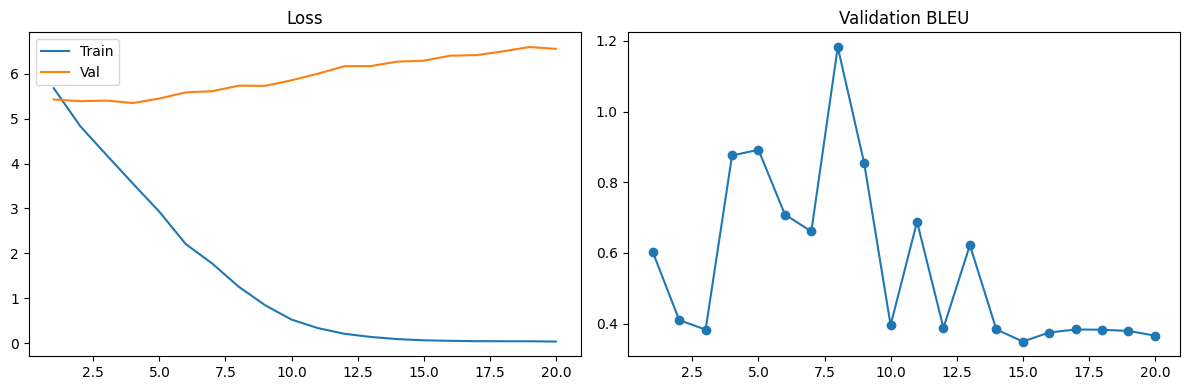
\includegraphics[keepaspectratio]{images/att1-loss-plot.png}}

Plot 2: Attempt 2 Training Trace

\pandocbounded{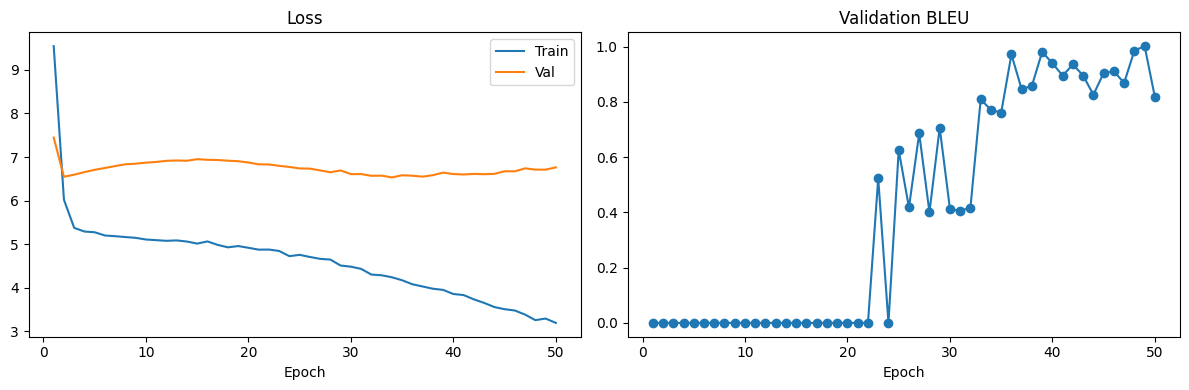
\includegraphics[keepaspectratio]{images/att2-loss-plot.png}}

Plot 3: Attempt 3 Training Trace

\pandocbounded{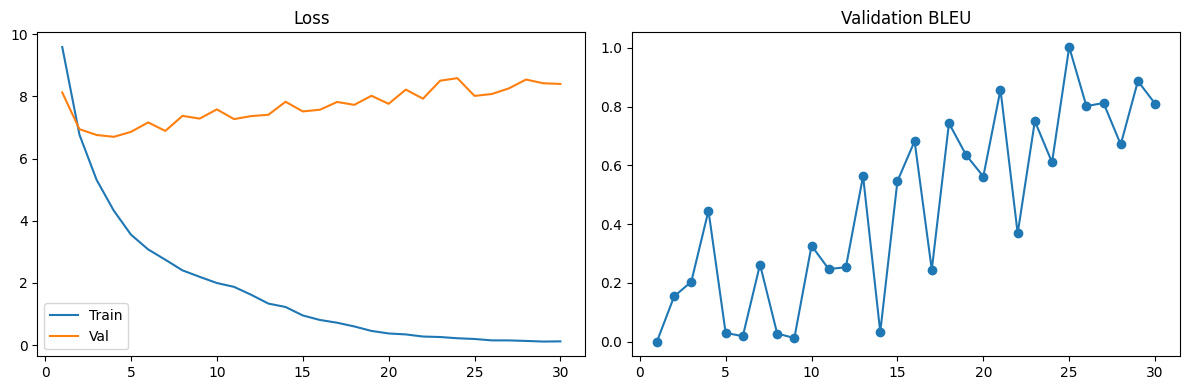
\includegraphics[keepaspectratio]{images/att3-loss-plot.png}}

Across all three NMT models, the training loss decrease monotonically,
indicating these algorithms's ability to fit our training data. In
contrast, as for the validation loss curves, three models all achieved
the lowest validation loss before epoch 5, which reflects the contraint
imposed by the size of our corpus. That same data size issue can explain
part of the unstable and spiky behavior for validation BLEU scores over
the training. Notably, in our attempt2, the manchuBERT-LSTM arrangement,
there seems to be an increasing trend in the validation BLEU score.

\subsubsection{Evaluation Metrics}\label{evaluation-metrics-1}

\begin{longtable}[]{@{}
  >{\raggedright\arraybackslash}p{(\linewidth - 6\tabcolsep) * \real{0.3418}}
  >{\raggedleft\arraybackslash}p{(\linewidth - 6\tabcolsep) * \real{0.1899}}
  >{\raggedleft\arraybackslash}p{(\linewidth - 6\tabcolsep) * \real{0.1899}}
  >{\raggedleft\arraybackslash}p{(\linewidth - 6\tabcolsep) * \real{0.2785}}@{}}
\toprule\noalign{}
\begin{minipage}[b]{\linewidth}\raggedright
Model / Approach
\end{minipage} & \begin{minipage}[b]{\linewidth}\raggedleft
Best (Val BLEU)
\end{minipage} & \begin{minipage}[b]{\linewidth}\raggedleft
Best (Val Loss)
\end{minipage} & \begin{minipage}[b]{\linewidth}\raggedleft
Longer Training Sample
\end{minipage} \\
\midrule\noalign{}
\endhead
\bottomrule\noalign{}
\endlastfoot
Seq2Seq (2 GRUs) & 2.08 & 0.72 & 0.94 \\
manchuBERT + LSTM & 1.38 & 1.27 & 1.44 \\
manchuBERT + mBART & 1.86 & 0.47 & 1.86 \\
\end{longtable}

To understand these BLEU scores, we can first look at the results scores
from the first three attempts, which involve model training. Under the
conventional validation set approach for model selection, choosing the
best model basing on validation loss, it is manchuBERT + LSTM model that
performs best. If we allow another way of assessing the model's ability
to extrapolate, the BLEU scores evaluated on the models with the best
BLEU score, then it is the baseline seq2seq network that outperforms
other two, this aligns with our understanding the relationship between
data size and the size of training parameters.

The other interesting observation is that the manchBERT + mBART model
arrangement, though makes a great sense for me, but when implementing I
wrestled with the tokenization alignment quite a bit only to get it
working and the training was very slow. This to a certain extent points
me to an understanding of model flexibility, that my third attempt was
the architecture is a bit grand and sophisticated for my 300 language
pairs.

Then comes to the performance of the fourth attempt. I am interested in
examining, provided linguistic knowlege and lexical meanings of the
words in a sentence alone, LLM's capability to do translation on
languages that they were not explicitly trained on. Thus, I design an
experiment with hope that I can to some extent eliminate the prior
knowledge of Manchu of LLM. Specifically, I referred to the Pei et
al.~paper(Pei, Liu, Lin, Yvon, and Schütze
(\citeproc{ref-pei2025understandingincontextmachinetranslation}{2025})),
and do a comparison between 4 conditions created by different prompt
configurations:

\begin{enumerate}
\def\labelenumi{\arabic{enumi}.}
\tightlist
\item
  Directly Translation with no dictionary resource and no source
  language information
\item
  The source language is not specified but dictionary entries are
  provided
\item
  Provide deliberately misnamed source language \texttt{Anchum} and the
  right dictionary entries
\item
  Source language is Manchu directly specified with dictionary entries
\end{enumerate}

\begin{longtable}[]{@{}
  >{\raggedright\arraybackslash}p{(\linewidth - 8\tabcolsep) * \real{0.2673}}
  >{\raggedleft\arraybackslash}p{(\linewidth - 8\tabcolsep) * \real{0.1485}}
  >{\raggedleft\arraybackslash}p{(\linewidth - 8\tabcolsep) * \real{0.1485}}
  >{\raggedleft\arraybackslash}p{(\linewidth - 8\tabcolsep) * \real{0.2178}}
  >{\raggedleft\arraybackslash}p{(\linewidth - 8\tabcolsep) * \real{0.2178}}@{}}
\toprule\noalign{}
\begin{minipage}[b]{\linewidth}\raggedright
****
\end{minipage} & \begin{minipage}[b]{\linewidth}\raggedleft
Explicitly Manchu-English + dict
\end{minipage} & \begin{minipage}[b]{\linewidth}\raggedleft
Misnaming source as Anchum + dict
\end{minipage} & \begin{minipage}[b]{\linewidth}\raggedleft
Source language not specified + dict
\end{minipage} & \begin{minipage}[b]{\linewidth}\raggedleft
Direct translation without dictionary
\end{minipage} \\
\midrule\noalign{}
\endhead
\bottomrule\noalign{}
\endlastfoot
In-context LLM + Dictionary & 4.47 & 1.65 & 1.77 & 1.44 \\
\end{longtable}

We can a spot a distinctively higher test BLEU score for the condition
which we not only provide lexical mappings in the prompt but also
specify explicitly that the task is to do Manchu-English translation.
While the performance drop when there is misinformation or no
information about the source language. However, from the generated
translations, we can see that LLM are good at forming fluent English
sentences given a bag of words and meanings, it can be suggested that
the BLEU score is underestimated due to the abundant verb conjugations
or suffixations in Manchu grammar, since when there exists words in the
sentence that don't have English definitions, the translation quality
drops.

\subsubsection{Translation Sample}\label{translation-sample}

Although BLEU is designed to be a more robust way to evaluate machine
translation, comparing to using the cross entropy loss alone, it's still
operating on the n-grams mindset. Regarding this limitation, I go for
the most intuitive way to examine translation quality, which is the
translation itself for the test set by different models. This leads me
to some interesting observations which would serve a good ending for the
evaluation section.

We can see that Attempt 4 (in-context LLM + Dict), generally yields
decent translations, nevetheless this approach is vulnerable when word
in a sentence did not find a mapping in our dictionary, such as in the
case of ID 4, ``loo tai tai''---a Manchu transliteration of a Chinese
meaning old lady, does not appear in the dictionary, but they are
mismatched to `LOO: prison; gong; cf.~lo; see lomi', `TAI: platform,
terrace, stage', thus drives the translation off the correct path.
Interestingly, for the same ID 4 sentence translation, Attempt
3(manchuBERT + mBART) somewhat capture the meaning of loo tai tai in the
sentence. The cases that the translation of Attempt 3 are
underestimated, ID 16 is one example, it almost captures the first hald
of the sentence, but later falls into decoder degeneration.

Attempt 1(2 GRUs) often produces fluent and syntactically well English
translation, and the translation often involve sensical phrases such as
``at all'' in ID 4 and ``at this early hour'' for ID 20 translation,
which aligns part of the sentence pretty well.

\begin{Shaded}
\begin{Highlighting}[]

\SpecialCharTok{==}\ErrorTok{============================}
\NormalTok{ID}\SpecialCharTok{:} \DecValTok{4}
\SpecialCharTok{==}\ErrorTok{============================}
\FunctionTok{SOURCE}\NormalTok{ (Manchu)}\SpecialCharTok{:}
\NormalTok{jiduji loo tai tai fulu kai}

\FunctionTok{REFERENCE}\NormalTok{ (English)}\SpecialCharTok{:}
\NormalTok{your venerable ladyship}
\SpecialCharTok{{-}{-}{-}{-}}\NormalTok{ attempt1\_seq2seq\_gru }\SpecialCharTok{{-}{-}{-}{-}}
\NormalTok{Sentence BLEU}\SpecialCharTok{:} \DecValTok{0}
\ControlFlowTok{if}\NormalTok{ you have been at all}
\SpecialCharTok{{-}{-}{-}{-}}\NormalTok{ attempt2\_manchubert\_lstm\_frozen }\SpecialCharTok{{-}{-}{-}{-}}
\NormalTok{Sentence BLEU}\SpecialCharTok{:} \DecValTok{0}
\NormalTok{we will be to the }\ControlFlowTok{in}\NormalTok{ of the}
\SpecialCharTok{{-}{-}{-}{-}}\NormalTok{ attempt3\_manchubert\_mbart }\SpecialCharTok{{-}{-}{-}{-}}
\NormalTok{Sentence BLEU}\SpecialCharTok{:} \DecValTok{0}
\NormalTok{where it is it will dear senior me}
\SpecialCharTok{{-}{-}{-}{-}}\NormalTok{ attempt4\_incontext\_dict }\SpecialCharTok{{-}{-}{-}{-}}
\NormalTok{Sentence BLEU}\SpecialCharTok{:} \DecValTok{0}
\NormalTok{after all the prison platforms are truly excellent}

\SpecialCharTok{==}\ErrorTok{============================}
\NormalTok{ID}\SpecialCharTok{:} \DecValTok{16}
\SpecialCharTok{==}\ErrorTok{============================}
\FunctionTok{SOURCE}\NormalTok{ (Manchu)}\SpecialCharTok{:}
\NormalTok{si absi erei gese sain arahabi}

\FunctionTok{REFERENCE}\NormalTok{ (English)}\SpecialCharTok{:}
\NormalTok{how is it you have written them so well}
\SpecialCharTok{{-}{-}{-}{-}}\NormalTok{ attempt1\_seq2seq\_gru }\SpecialCharTok{{-}{-}{-}{-}}
\NormalTok{Sentence BLEU}\SpecialCharTok{:} \FloatTok{7.45}
\NormalTok{you have been}
\SpecialCharTok{{-}{-}{-}{-}}\NormalTok{ attempt2\_manchubert\_lstm\_frozen }\SpecialCharTok{{-}{-}{-}{-}}
\NormalTok{Sentence BLEU}\SpecialCharTok{:} \FloatTok{17.87}
\NormalTok{how is it it it}
\SpecialCharTok{{-}{-}{-}{-}}\NormalTok{ attempt3\_manchubert\_mbart }\SpecialCharTok{{-}{-}{-}{-}}
\NormalTok{Sentence BLEU}\SpecialCharTok{:} \FloatTok{19.49}
\NormalTok{how is it that you how is it}
\SpecialCharTok{{-}{-}{-}{-}}\NormalTok{ attempt4\_incontext\_dict }\SpecialCharTok{{-}{-}{-}{-}}
\NormalTok{Sentence BLEU}\SpecialCharTok{:} \FloatTok{12.26}
\NormalTok{how well you have made it like this}
\end{Highlighting}
\end{Shaded}

\begin{Shaded}
\begin{Highlighting}[]
\SpecialCharTok{==}\ErrorTok{============================}
\NormalTok{ID}\SpecialCharTok{:} \DecValTok{20}
\SpecialCharTok{==}\ErrorTok{============================}
\FunctionTok{SOURCE}\NormalTok{ (Manchu)}\SpecialCharTok{:}
\NormalTok{enteke erde uthai feksime jifi ainambi}

\FunctionTok{REFERENCE}\NormalTok{ (English)}\SpecialCharTok{:}
\NormalTok{what have you run over to do at this early hour}
\SpecialCharTok{{-}{-}{-}{-}}\NormalTok{ attempt1\_seq2seq\_gru }\SpecialCharTok{{-}{-}{-}{-}}
\NormalTok{Sentence BLEU}\SpecialCharTok{:} \FloatTok{26.3}
\ControlFlowTok{if}\NormalTok{ you have been at this early hour}
\SpecialCharTok{{-}{-}{-}{-}}\NormalTok{ attempt2\_manchubert\_lstm\_frozen }\SpecialCharTok{{-}{-}{-}{-}}
\NormalTok{Sentence BLEU}\SpecialCharTok{:} \FloatTok{4.41}
\NormalTok{how is it that you have it}
\SpecialCharTok{{-}{-}{-}{-}}\NormalTok{ attempt3\_manchubert\_mbart }\SpecialCharTok{{-}{-}{-}{-}}
\NormalTok{Sentence BLEU}\SpecialCharTok{:} \FloatTok{7.5}
\NormalTok{you have you but you have come back again }\ControlFlowTok{for}\NormalTok{ me}
\SpecialCharTok{{-}{-}{-}{-}}\NormalTok{ attempt4\_incontext\_dict }\SpecialCharTok{{-}{-}{-}{-}}
\NormalTok{Sentence BLEU}\SpecialCharTok{:} \FloatTok{4.52}
\NormalTok{why are you coming leaping so early }\ControlFlowTok{in}\NormalTok{ the morning}
\end{Highlighting}
\end{Shaded}

\subsection{Discussion}\label{discussion}

In general, all machine translation attempts in this project show low
BLEU scores, which is expected in terms of the obvious discrepancy
between the millions of parameters these models have and the very modest
size of my dataset. \textbf{Low-resource NMT} has become a very popular
reseach area recently, this project explored many of the proposed
remedies, leaving others not reached, in doing so to some degree tested
the practical boundaries of what counts as low-resource language. Many
languages described as ``low-resource'' in the NLP literature still
possess orders of magnitude more data than Manchu, which has almost no
modern digital presence.\footnote{low relatively to French-English,
  Spanish-English pairs}

However, this practice and seeing it as a concrete appreciation of the
obstacles of data scaricity in a NMT model, is meaningful to me because
I finally get to go from not just vaguely think about how I can use data
science to preserve Manchu but to actually get a neural machine
translation model working. And throughout this project, I was able to
familiarize myself with where the exisiting resource are, and started
thinking about what resource I can potentially introduce. In addition,
getting to meet these communities dedicating to Manchu preservation with
their research effort was in itself very instructive and motivating.

\phantomsection\label{refs}
\begin{CSLReferences}{1}{0}
\bibitem[\citeproctext]{ref-caoHungLouMeng2006}
Cao, Xueqin. 2006. \emph{Hung {Lou Meng}, or, the {Dream} of the {Red
Chamber}, a {Chinese Novel}, {Book I}}. Translated by H. Bencraft Joly.

\bibitem[\citeproctext]{ref-leeManNERManPOSPioneering2024}
Lee, Sangah, Sungjoo Byun, Jean Seo, and Minha Kang. 2024. {``{ManNER}
\& {ManPOS}: {Pioneering NLP} for Endangered {Manchu} Language.''} In
\emph{Proceedings of the 2024 {Joint International Conference} on
{Computational Linguistics}, {Language Resources} and {Evaluation}
({LREC-COLING} 2024)}, 11030--39.

\bibitem[\citeproctext]{ref-liuMultilingualDenoisingPretraining2020}
Liu, Yinhan, Jiatao Gu, Naman Goyal, Xian Li, Sergey Edunov, Marjan
Ghazvininejad, Mike Lewis, and Luke Zettlemoyer. 2020. {``Multilingual
{Denoising Pre-training} for {Neural Machine Translation}.''} Edited by
Mark Johnson, Brian Roark, and Ani Nenkova. \emph{Transactions of the
Association for Computational Linguistics} 8: 726--42.
\url{https://doi.org/10.1162/tacl_a_00343}.

\bibitem[\citeproctext]{ref-NLPScratchTranslation}
{``{NLP From Scratch}: {Translation} with a {Sequence} to {Sequence
Network} and {Attention} --- {PyTorch Tutorials} 2.9.0+cu128
Documentation.''} n.d.
https://docs.pytorch.org/tutorials/intermediate/seq2seq\_translation\_tutorial.html.
Accessed December 15, 2025.

\bibitem[\citeproctext]{ref-normanComprehensiveManchuEnglishDictionary2013}
Norman, Jerry. 2013. \emph{A {Comprehensive Manchu-English Dictionary}}.
Cambridge, MA, UNITED STATES: Harvard University Asia Center.

\bibitem[\citeproctext]{ref-pei-etal-2025-understanding}
Pei, Renhao, Yihong Liu, Peiqin Lin, François Yvon, and Hinrich
Schuetze. 2025. {``Understanding in-Context Machine Translation for
Low-Resource Languages: A Case Study on {M}anchu.''} In
\emph{Proceedings of the 63rd Annual Meeting of the Association for
Computational Linguistics (Volume 1: Long Papers)}, edited by Wanxiang
Che, Joyce Nabende, Ekaterina Shutova, and Mohammad Taher Pilehvar,
8767--88. Vienna, Austria: Association for Computational Linguistics.
\url{https://doi.org/10.18653/v1/2025.acl-long.429}.

\bibitem[\citeproctext]{ref-pei2025understandingincontextmachinetranslation}
Pei, Renhao, Yihong Liu, Peiqin Lin, François Yvon, and Hinrich Schütze.
2025. {``Understanding in-Context Machine Translation for Low-Resource
Languages: A Case Study on Manchu.''}
\url{https://arxiv.org/abs/2502.11862}.

\bibitem[\citeproctext]{ref-seoMergenFirstManchuKorean2024}
Seo, Jean, Sungjoo Byun, Minha Kang, and Sangah Lee. 2024. {``Mergen:
{The First Manchu-Korean Machine Translation Model Trained} on
{Augmented Data},''} no. arXiv:2311.17492 (January).
\url{https://doi.org/10.48550/arXiv.2311.17492}.

\bibitem[\citeproctext]{ref-CaoXueQinHongLouMengXiBoWen1993}
曹雪芹穆旭東. 1993. \emph{{红楼梦(锡伯文)}}. 新疆人民出版社.

\end{CSLReferences}




\end{document}
